\newpage
\section{Introduction}
\label{sec:Introduction}
With the rise of deep learning in image processing \ac{SR} and \ac{IC}
in both the image and the video domain have received significant
attention \cite{DLFISRAS}. While SR aims to reconstruct a \ac{HR} from a
\ac{LR}, image colorization deals with the transformation from an uncolored,
\ac{GRY} to a RGB \ac{COL}.
However, in most of the recent works (e.g. \cite{AFPATSISR}, \cite{ESRGAN},
\cite{RBPNFVSR}, \cite{LFVSRTHROFE}) the problem of downscaling and upscaling
or decolorization and colorization are regarded as seperate problems although
upscaling often is preceded by downscaling, leading to a loss of information
from the downscaling process which makes the inverse problem of SR highly
ill-posed \cite{TAID}. Despite of the large progress in SR in the last years
(\cite{DLFISRAS}) very specific details therefore often cannot be reconstructed,
when interpolation is used for downsampling. However, as shown in
\myfigref{fig:shrb_vs_shrt_x4} the downsampling method has a large impact on
the performance of the subsequent upscaling task.

\begin{figure}[!htbp]
\centering
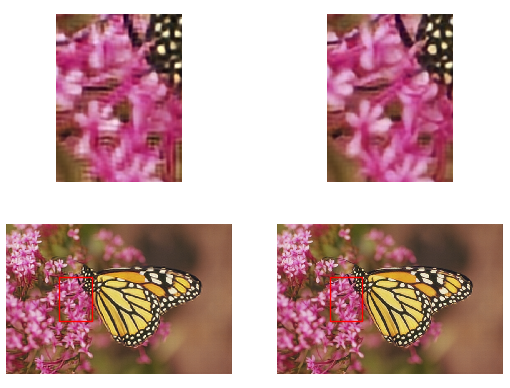
\includegraphics[width=10cm]{figures/shrb_vs_shrt_x4}
\caption{Comparison between an upscaled image based on bicubic downsampled
(left) and task aware downsampled (right) LR image applied on the same model
with upscaling factor 4.}
\label{fig:shrb_vs_shrt_x4}
\end{figure}

As can be seen above a task aware approach can dramatically improve the
performance of existing super-resolution models in terms of reconstruction
quality while keeping the compression rate constant. However, the research on task
aware downscaling methods is a very new field and therefore there still are
a lot of unresolved issues such as the effect of perturbation or the feasibility of
applying it to tasks other than \ac{SISR} and \ac{IC}.

\subsection{Focus of this Work}
For this reason this work focuses on \ac{TAD} for several standard
computer vision problems such as super-resolution or colorization in both the
image and video domain, as recently purposed by Heewon Kim et. alt. (\cite{TAID})
for the image domain only. However, as shown in \myfigref{fig:taid_problems}
the \ac{TAD} implementation purposed in \cite{TAID} suffers from vulnerability
against perturbation of the downscaled image. Although the purposed model is
quite shallow having 10 convolutions for each scaling process only, there still
is potential for improvement, which especially gains importance when \ac{TAD} is
applied to the video domain (for real-time capabilites).

\begin{figure}[!htbp]
\centering

\includegraphics[width=10cm]{figures/cvl}
\caption{Problems of task aware downscaling as purposed by \cite{TAID}:
Perturbation (left), Runtime (right)}
\label{fig:taid_problems}
\end{figure}

Therefore the goals of this work are the following:

\begin{itemize}
\item reimplement and evaluate the \ac{TAD} framework purposed in (\cite{TAID})
\item improve the \ac{TAD} framework especially with regards on the trade-off
between model-complexity (runtime) and restoring quality (PSNR) as well as
with regards on robustness against perturbations
\item extend the \ac{TAD} framework to the video domain
\end{itemize}

By that to the best of our knowledge this work is the first one using deep
learning for downscaling in the video domain.

\subsection{Thesis Organization}
After the problem statement \mychapterref{sec:Introduction} related works are
introduced for both the image and video domain \mychapterref{sec:RelatedWork}.
\mychapterref{sec:Approach} explains the methods that are used in order to
achieve the goals described above and which are evaluated in
\mychapterref{sec:ExperimentsandResults}. A final discussion of the results
as well as an outlook on further work can be found in
\mychapterref{sec:Discussion}. Further visualization and experiments are
shown in the abstract.

% Give an introduction to the topic you have worked on:
%
% \begin{itemize}
%  \item \textit{What is the rationale for your work?} Give a sufficient description of the problem, e.g. with a general description of the problem setting, narrowing down to the particular problem you have been working on in your thesis. Allow the reader to understand the problem setting.
%  \item \textit{What is the scope of your work?} Given the above background, state briefly the focus of the work, what and how you did.
%  \item \textit{How is your thesis organized?} It helps the reader to pick the interesting points by providing a small text or graph which outlines the organization of the thesis. The structure given in this document shows how the general structuring shall look like. However, you may fuse sections or change their names according to the requirements of your thesis.
% \end{itemize}
